\documentclass{beamer}
\usetheme{Warsaw}
\usecolortheme{seahorse}

\usefonttheme[onlymath]{serif}

\usepackage{amsmath} 
\usepackage{bm}
\usepackage{graphicx}
\usepackage{tikz}
\usepackage{makecell}
\usepackage{listofitems}
\usepackage{media9}
\usepackage{multimedia}
\usepackage{comment}
\usepackage[separate-uncertainty = true]{siunitx}
\usepackage[style=numeric,backend=bibtex,sorting=none]{biblatex}
\usepackage[outline]{contour}

\usetikzlibrary{positioning}

\setbeamertemplate{navigation symbols}{}

\setbeamerfont{bibliography item}{size=\tiny}
\setbeamerfont{bibliography entry author}{size=\tiny}
\setbeamerfont{bibliography entry title}{size=\tiny}
\setbeamerfont{bibliography entry location}{size=\tiny}
\setbeamerfont{bibliography entry note}{size=\tiny}

\addbibresource{citations.bib}

\nocite{*}

\newcommand\blfootnote[1]{
	\begingroup
	\renewcommand\thefootnote{}\footnote{#1}
	\addtocounter{footnote}{-1}
	\endgroup
}

\tikzset{
	bn/.style={draw, rectangle, fill=blue!20, rounded corners},
	on/.style={draw, rectangle, fill=orange!20, rounded corners},
	rn/.style={draw, rectangle, fill=red!20, rounded corners},
	to/.style={->, >=stealth, thick}
}

\title{Simulation studies of the ePIC Silicon Vertex Tracker}
\author{Candidate Number: 1077795}

\begin{document}
\begin{frame}[plain]
    \maketitle
\end{frame}


\begin{frame}{Motivation}
	\begin{itemize}
		\item Tracking: Reconstructing path of particles from detector hits
		\item Allows for measurement of momentum and vertex positions
		\item Detector design decisions affect resolution so early simulations are very important
		\item The ePIC (Electron-Proton/Ion Collider) experiment needs a high precision silicon tracking detector
	\end{itemize}
	
	\begin{figure}
		\centering
		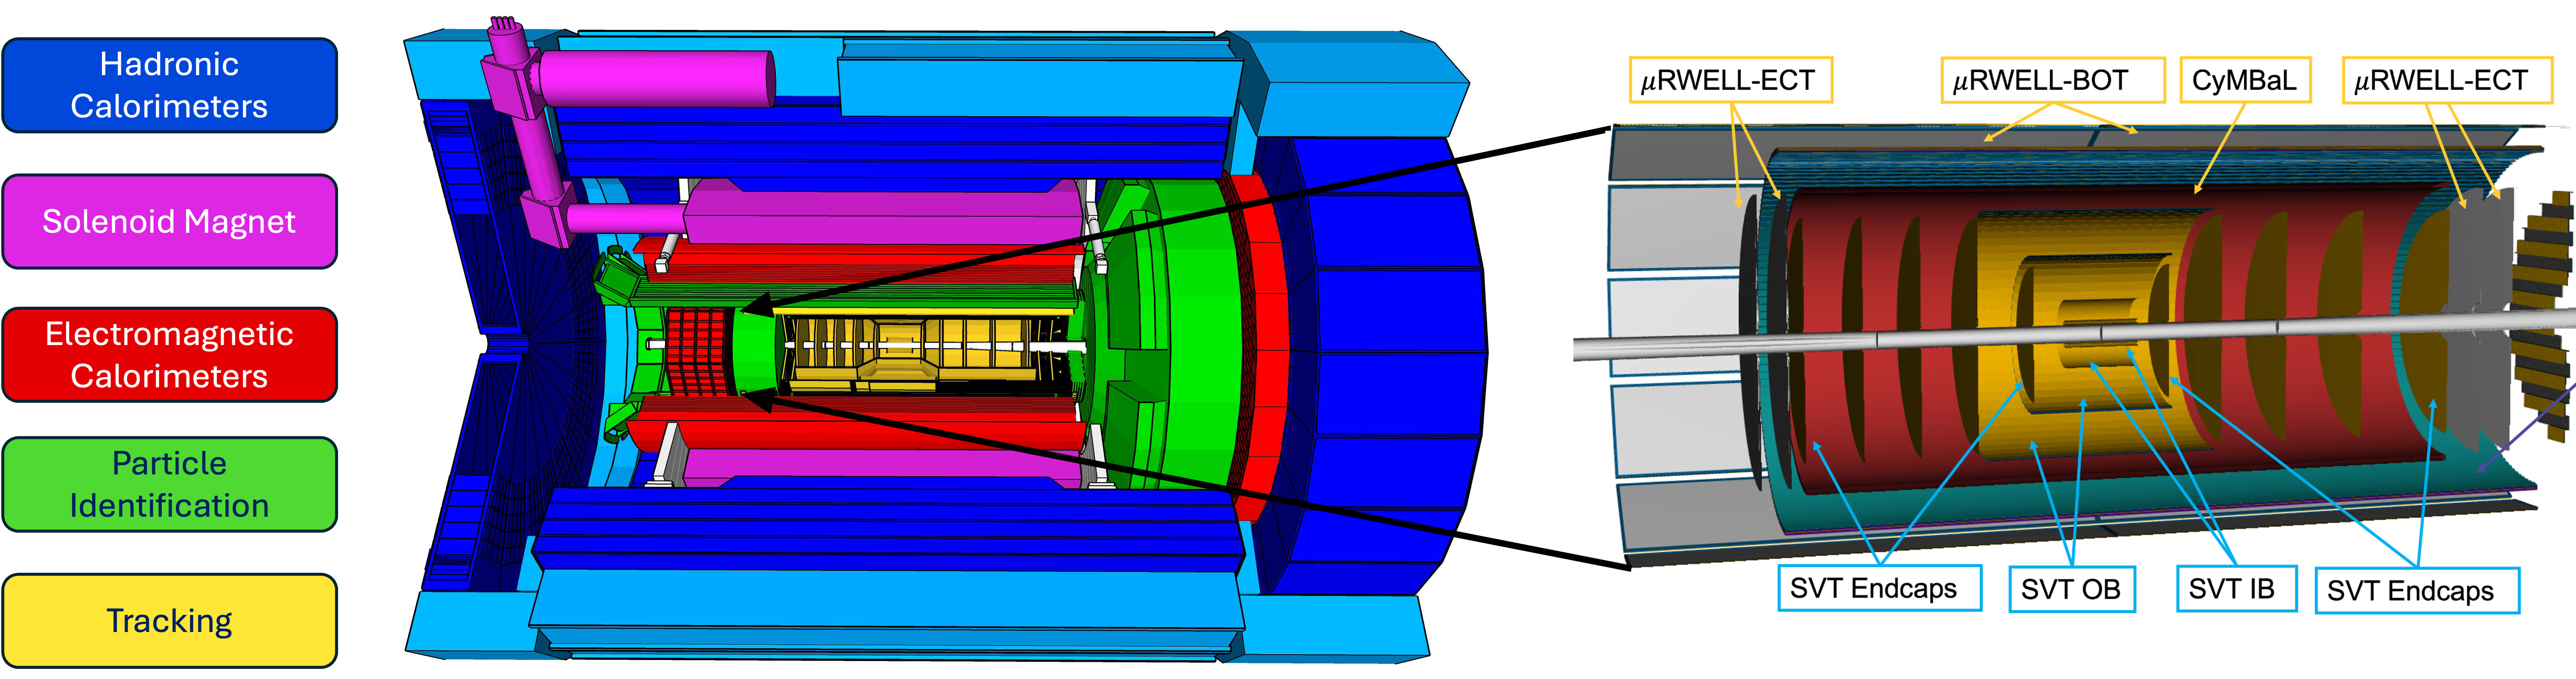
\includegraphics[width=0.8\linewidth]{epic_SVT_diagram}
		\label{fig:epicsvtdiagram}
		\caption{ePIC central detector, with tracking detectors highlighted} 
	\end{figure}
\end{frame}

\begin{frame}{Project overview}
	
	\begin{columns}
		\begin{column}{0.5\textwidth}
			
			\begin{itemize}
				\item Aim: Construct a simplified simulation of the ePIC Silicon Vertex Tracker (SVT), and evaluate the tracking performance for different detector parameters
				\item Simulations use Geant4, a C++ toolkit for simulating the passage of particles through matter using Monte Carlo methods
			\end{itemize}
		\end{column}
		\begin{column}{0.5\textwidth}
			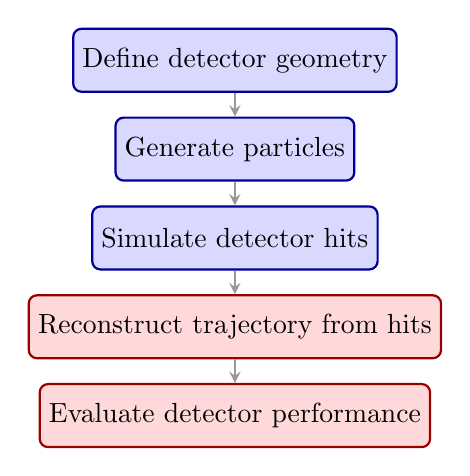
\begin{tikzpicture}[
				box/.style={
					draw, 
					rectangle, 
					rounded corners=3pt, 
					align=center,      
					minimum height=0.8cm,
					thick
				},
				sim/.style={box, fill=blue!15, draw=blue!60!black},
				ana/.style={box, fill=red!15, draw=red!60!black},
				arrow/.style={->, >=stealth, thick, draw=gray!80}
				]
				
				\node[sim] (a) {Define detector geometry};
				\node[sim, below=0.3cm of a] (b) {Generate particles};
				\node[sim, below=0.3cm of b] (c) {Simulate detector hits};
				
				\node[ana, below=0.3cm of c] (d) {Reconstruct trajectory from hits};
				\node[ana, below=0.3cm of d] (e) {Evaluate detector performance};
				
				\draw[arrow] (a) -- (b);
				\draw[arrow] (b) -- (c);
				\draw[arrow] (c) -- (d); 
				\draw[arrow] (d) -- (e);
				
			\end{tikzpicture}
		\end{column}
	\end{columns}

\end{frame}

\begin{frame}{Detector geometry}
	\begin{figure}
		\centering
		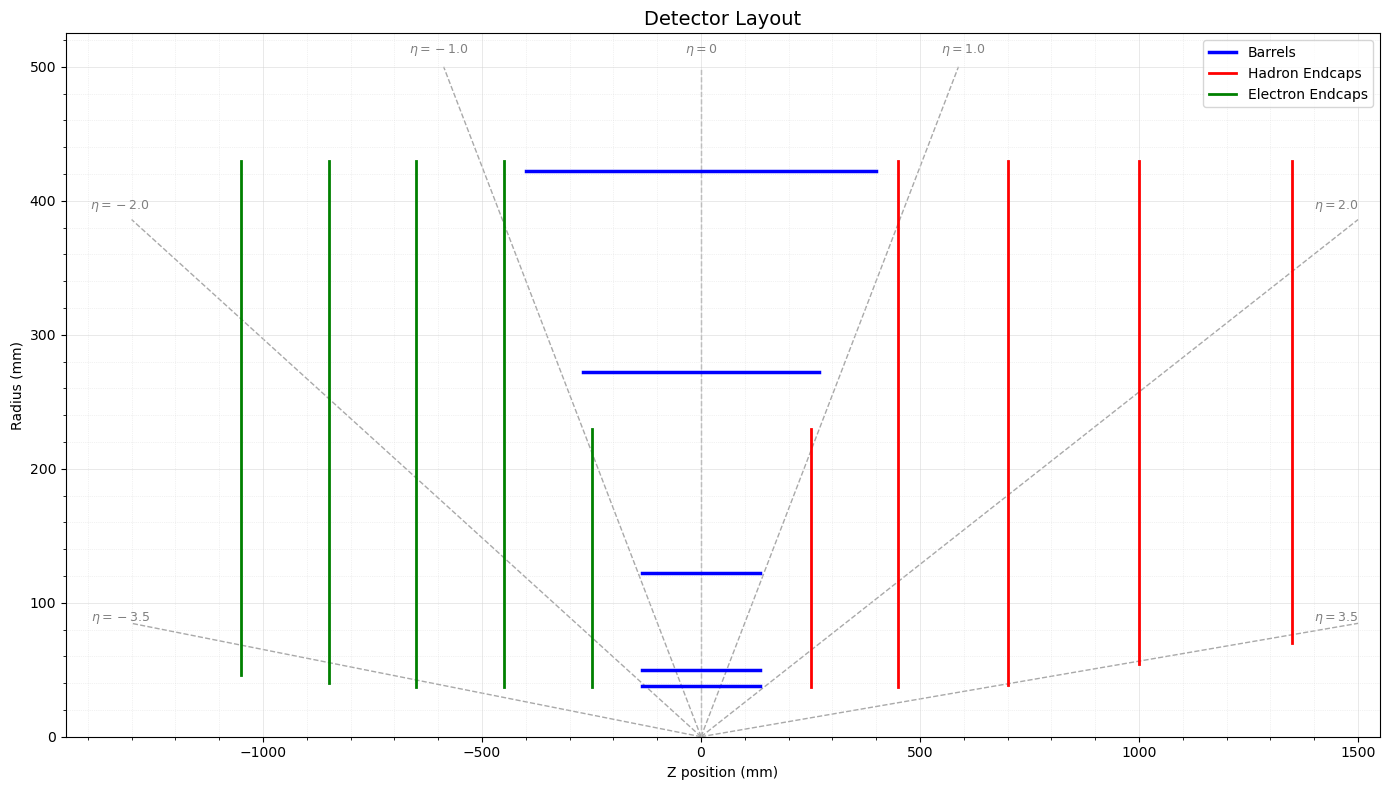
\includegraphics[width=0.85\linewidth]{detector_layout}
		\label{fig:detectorlayout}
	\end{figure}
	
	\begin{itemize}
		\item 3 Inner Barrel layers, 2 Outer Barrel layers, 10 endcap discs
		\item Also include copper layers to simulate support material, beryllium beampipe, and \SI{1.7}{\tesla} uniform magnetic field
	\end{itemize}
\end{frame}


\begin{frame}{Particle generation}
	\begin{figure}
		\centering
		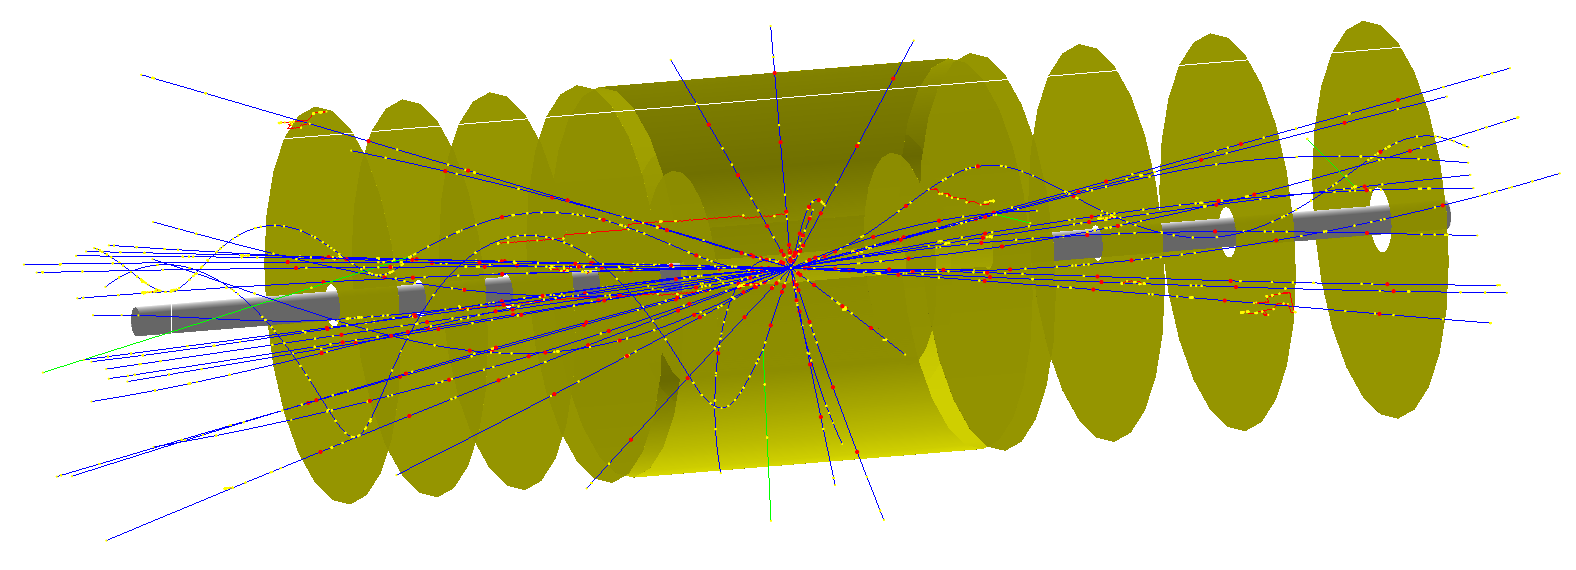
\includegraphics[width=1\linewidth]{geant4_screenshot}
		\caption{Screenshot of Geant4 simulation of detector with 50 pions}
		\label{fig:geant4screenshot}
	\end{figure}
	\begin{itemize}
		\item Positive pions were generated one at a time from the origin
		\item Pions chosen as they are the most common final state charged particle for electron-proton collisions at these energies
	\end{itemize}

\end{frame}

\begin{frame}{Detector hits}
	\begin{figure}
		\centering
		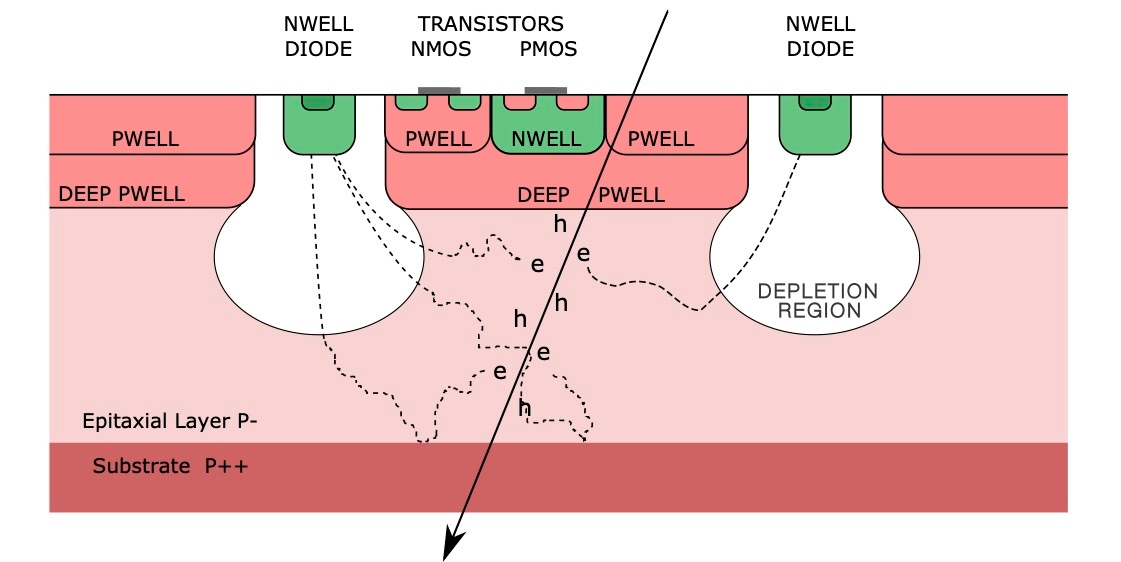
\includegraphics[width=0.7\linewidth]{MAPS_diagram}
		\caption{Schematic diagram of a Monolithic Active Pixel Sensor}
		\label{fig:mapsdiagram}
	\end{figure}
	
	\begin{itemize}
		\item Only register hits from primary pions, no secondary particles
		\item Apply a random Gaussian smearing to the hit position, with uncertainty $\sigma = $ \SI{7}{\micro \metre}, to simulate effect of finite pixel size, charge diffusion and pixel clustering 
	\end{itemize}
\end{frame}

\begin{comment}
	\begin{frame}{Parameterisation of helical trajectories}
		\begin{itemize}
			\item $d_0$: transverse distance in the $xy$-plane to the z-axis at the point of closest approach (POCA)
			\item $z_0$: is the z coordinate at the POCA
			\item $\phi_0$: azimuthal angle of the momentum vector at the POCA
			\item $p_T$: transverse momentum in the $xy$-plane, related to radius of circular motion $R = \frac{p_T}{qB}$
			\item $\tan \lambda$: tangent of the angle $\lambda$ between the momentum and the $xy$-plane
		\end{itemize}
		\begin{figure}
			\centering
			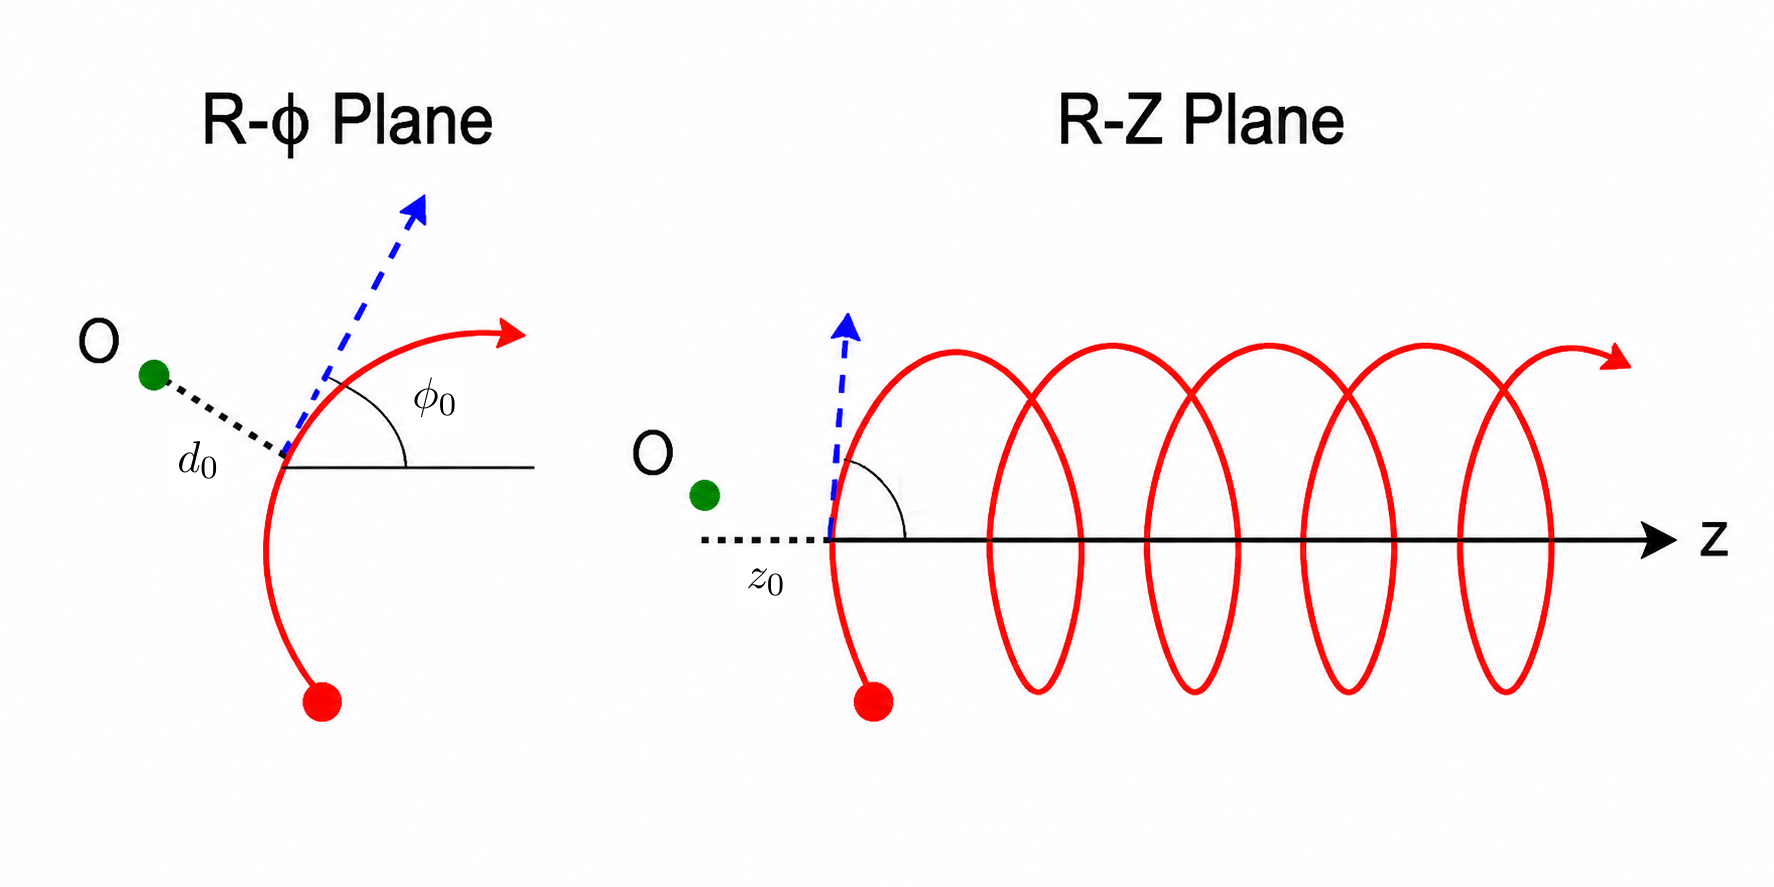
\includegraphics[width=0.85\linewidth]{helical_trajectory}
			\label{fig:helicaltrajectory}
		\end{figure}
	\end{frame}
\end{comment}

\begin{frame}{Track reconstruction}
	\begin{columns}
		\begin{column}{0.5\textwidth}
			\begin{figure}
				\centering
				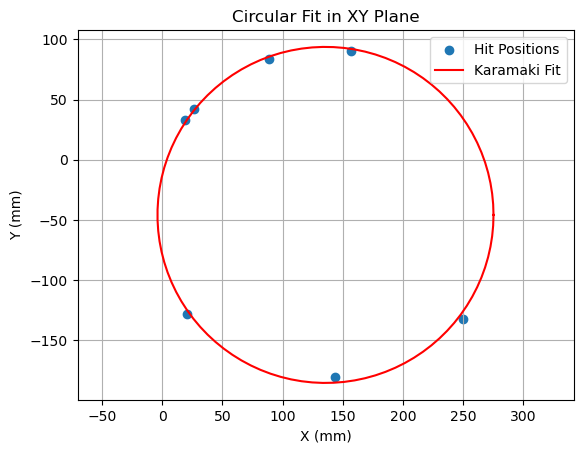
\includegraphics[width=1\linewidth]{circular_fit}
				\label{fig:circularfit}
			\end{figure}
		\end{column}
		\begin{column}{0.5\textwidth}
			\begin{figure}
				\centering
				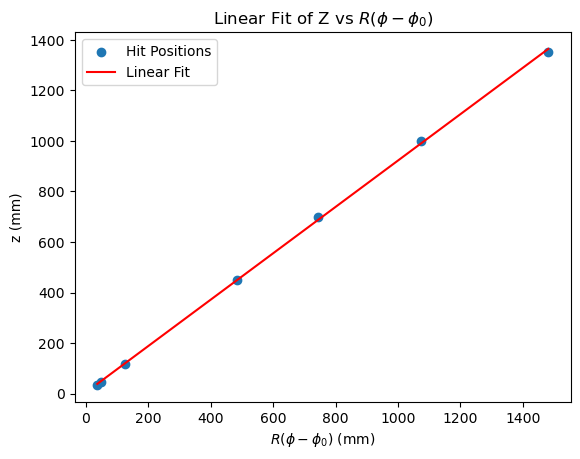
\includegraphics[width=1\linewidth]{linear_fit}
				\label{fig:linearfit}
			\end{figure}
		\end{column}
	\end{columns}
	
	\begin{itemize}
		\item Charged particles in a magnetic field move in a helical trajectory
		\item Fit a circle to the $xy$-positions, and linearly fit $z$ against the azimuthal angle of the momentum
		\item From these fitted parameters, we can determine the original position and momentum
	\end{itemize}
\end{frame}

\begin{frame}{Track reconstruction}
	\begin{figure}
		\centering
		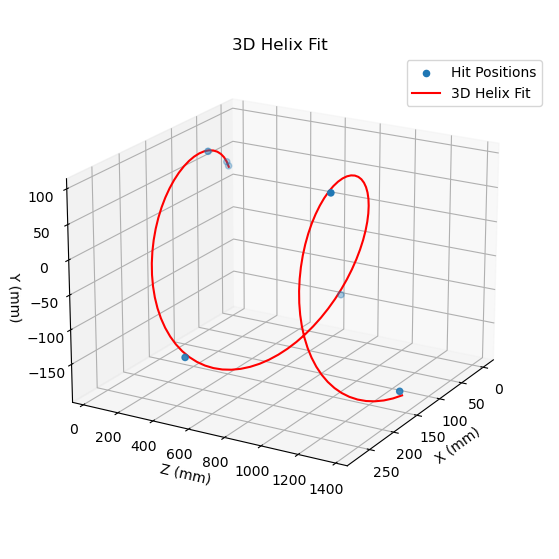
\includegraphics[width=0.8\linewidth]{helical_fit}
		\label{fig:helicalfit}
	\end{figure}
\end{frame}

\begin{frame}{Measuring tracking resolution}
	\begin{columns}
		\begin{column}{0.6\textwidth}
			\begin{figure}
				\centering
				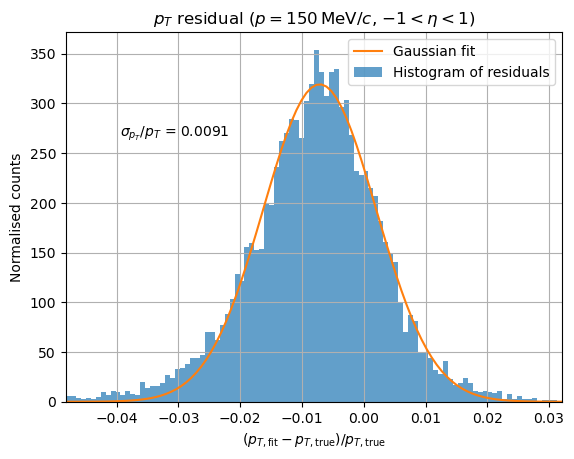
\includegraphics[width=1\linewidth]{gaussian_histogram_fit}
				\label{fig:gaussianhistogramfit}
			\end{figure}
		\end{column}
		\begin{column}{0.4\textwidth}
			Residuals: 
			\begin{itemize}
				\item Momentum: $\frac{p_{\mathrm{fit}} - p_{\mathrm{true}}}{p_{\mathrm{true}}}$ 
				\item Position: $x_{\mathrm{fit}} - x_{\mathrm{true}}$
			\end{itemize}
		\end{column}
	\end{columns}

	Simulate n=5,000,000 pion tracks, plot histogram of residual, fit Gaussian and extract uncertainty

\end{frame}

\begin{comment}
\begin{frame}{Sources of tracking uncertainty}
	\begin{itemize}
		\item Multiple Coulomb scattering results in many small deviations to the trajectory, with a long tailed distribution for total scattered angle
		\item Multiple scattering is sensitive to the material thickness and is worse for low momentum
		\item Low momentum: momentum resolution is dominated by multiple scattering, $\frac{\sigma_{p_T}}{p_T} \propto \frac{1}{p}$
		\item High momentum: momentum resolution is dominated by intrinsic detector uncertainty, $\frac{\sigma_{p_T}}{p_T} \propto p$
	\end{itemize}
\end{frame}
\end{comment}

\begin{frame}{Tracking resolution vs hit resolution}
	\begin{figure}
		\centering
		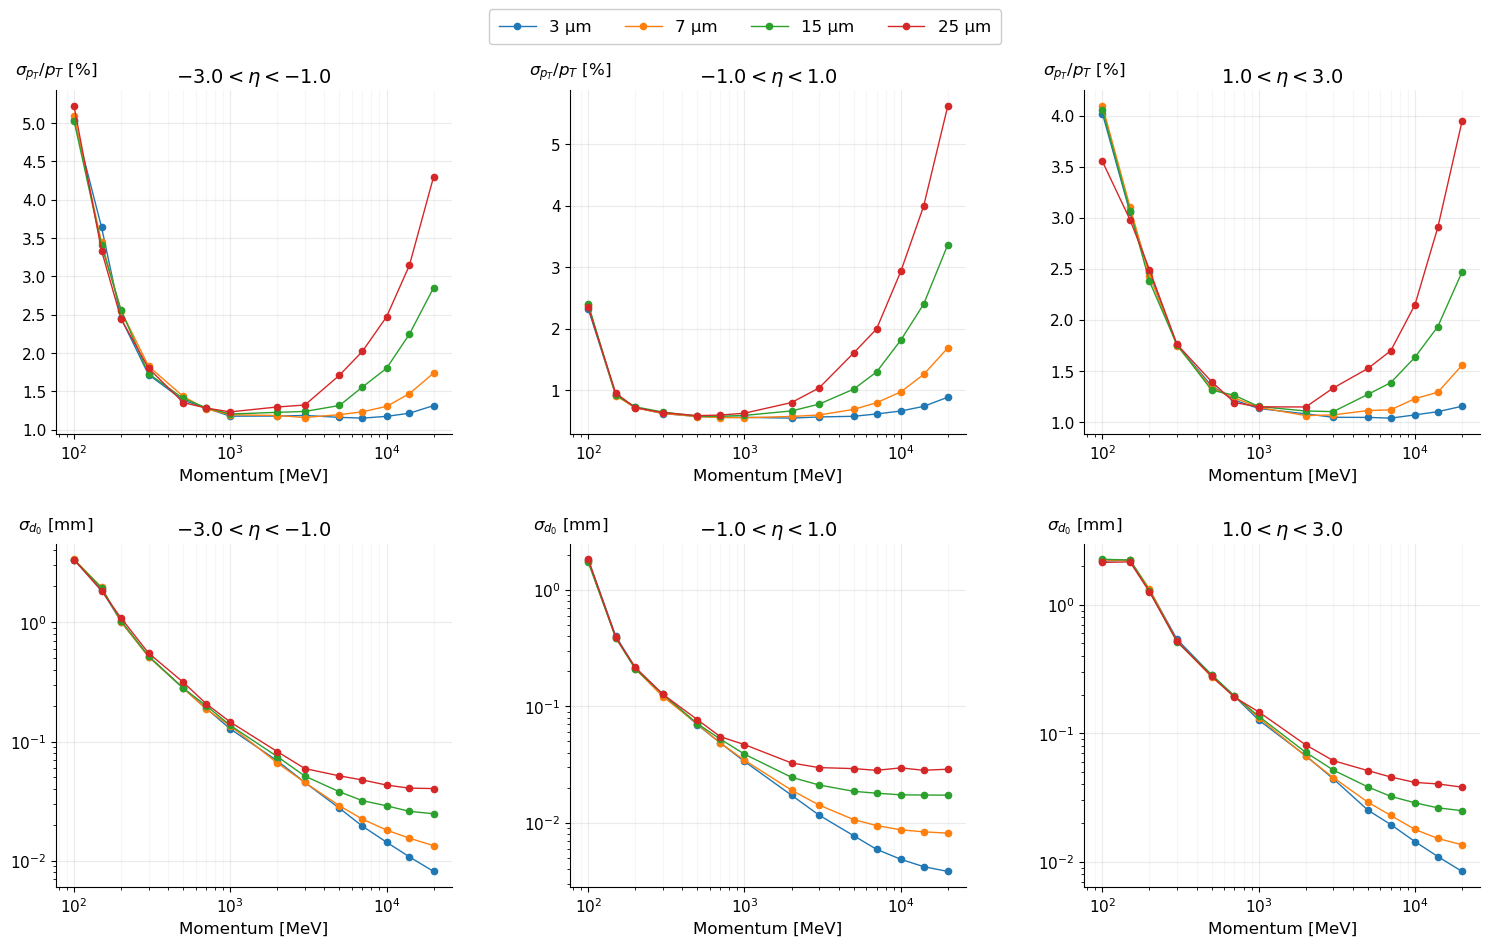
\includegraphics[width=0.9\linewidth]{resolution_vs_resolution}
		\label{fig:resolutionvsresolution}
	\end{figure}
	Intrinsic detector uncertainty affects resolution at large momentum
\end{frame}

\begin{frame}{Tracking resolution vs material thickness}
	\begin{figure}
		\centering
		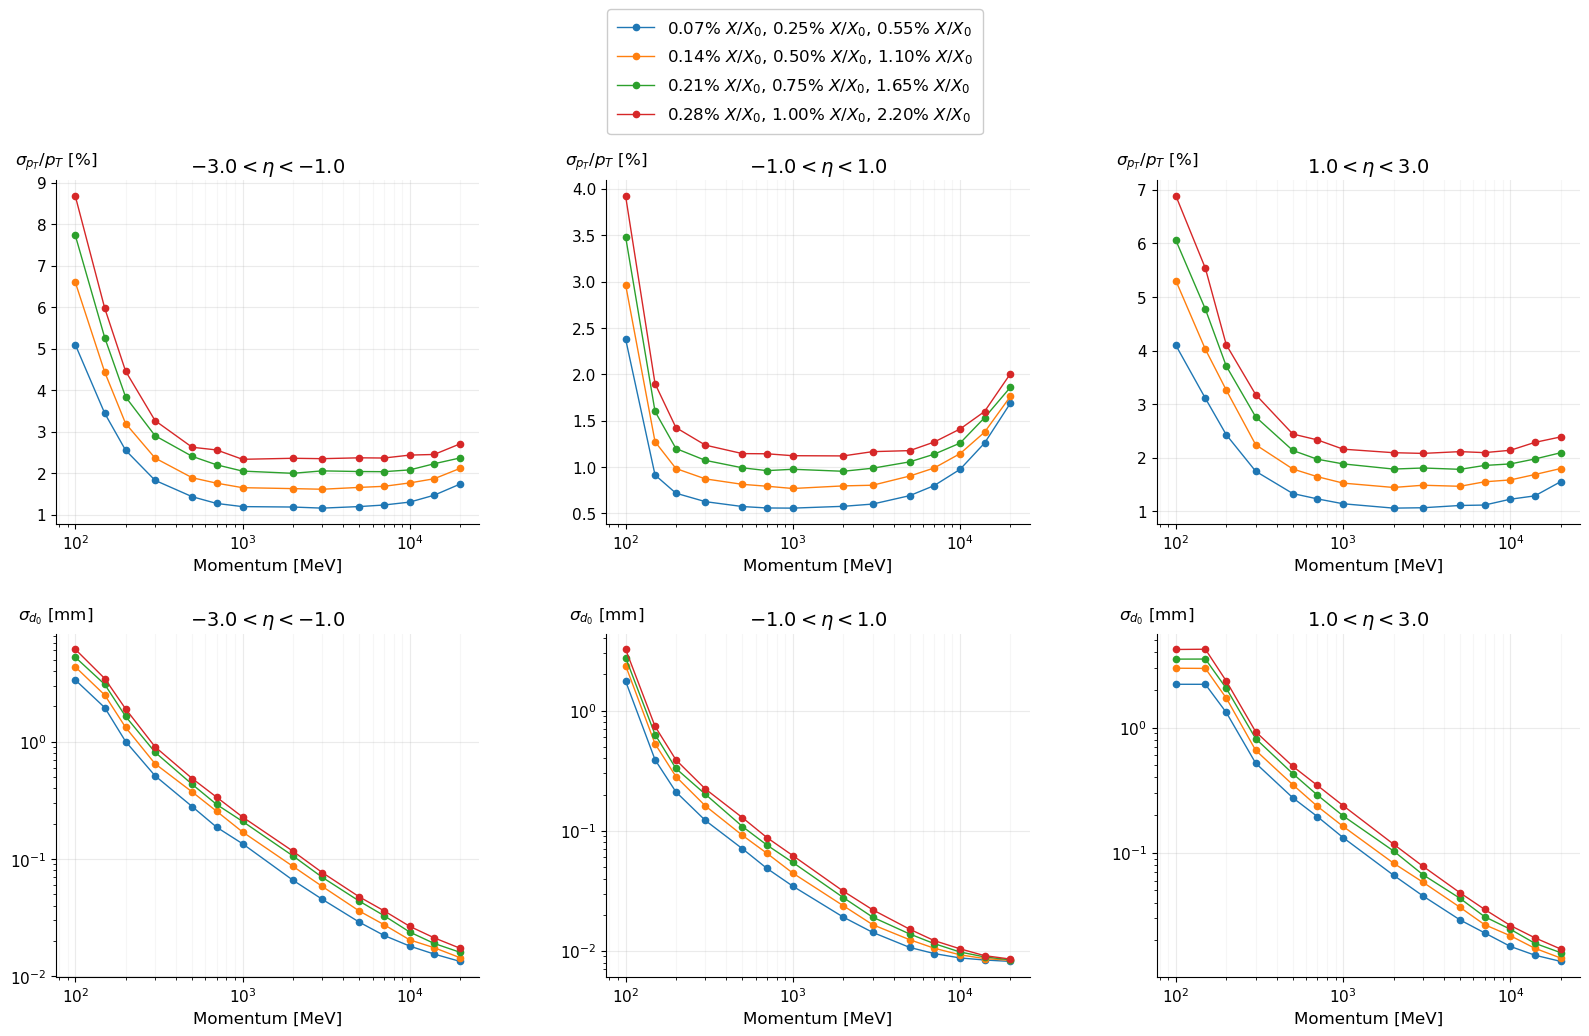
\includegraphics[width=0.9\linewidth]{resolution_vs_thickness}
		\label{fig:resolutionvsthickness}
	\end{figure}
	Material thickness strongly affects resolution across all momenta
\end{frame}

\begin{frame}{Tracking resolution vs magnetic field}
	\begin{figure}
		\centering
		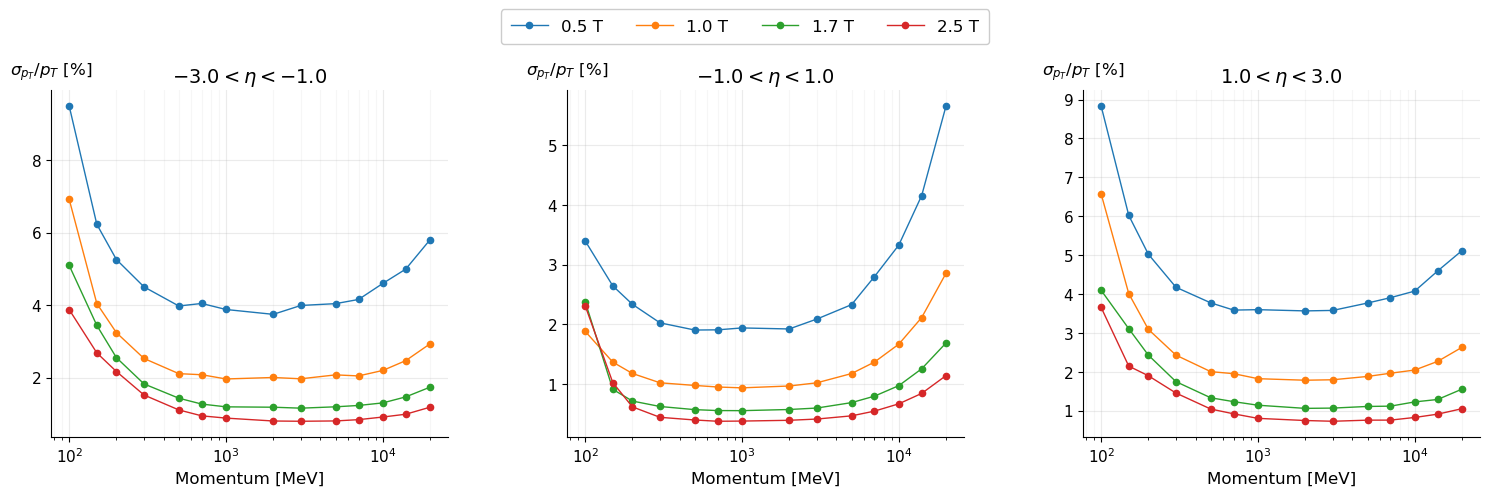
\includegraphics[width=1\linewidth]{resolution_vs_B}
		\label{fig:resolutionvsB}
	\end{figure}
	Magnetic field affects momentum resolution, but not position resolution 
\end{frame}

\begin{frame}{Future work}
	\begin{itemize}
		\item More realistic geometry, magnetic field and hit digitisation model
		\item Use track finding algorithms to study realistic collision scenarios (matching hits to tracks)
		\item Test more sophisticated tracking algorithms e.g. Kalman Filters
		\item Investigate alterations to detector geometry, such as changing number, position, or shape of layers
	\end{itemize}
\end{frame}

\end{document}
